\documentclass[12pt]{article}
\usepackage[english,greek]{babel}
\usepackage[utf8x]{inputenc}
\usepackage{graphicx}
\begin{document}


\title{Έγγραφο Aπαιτήσεων Λογισμικού \\
Εγγεγραμμένοι Χρήστες}
\date{\today}
\author{$Javengers$}
\maketitle

\tableofcontents

\clearpage

\section{Εισαγωγή}

\subsection{Ταυτότητα-Επιχειρησιακοί Στόχοι}


Ο στόχος των χρηστών-εθελοντών, δηλαδή των χρηστών που έχουν δημιουργήσει λογιαρισμό στη διαδικτυακή μας πλατφόρμα, είναι η εξοικονόμηση χρόνου και χρημάτων μέσω της αποτελεσματικής και αποδοτικής εύρεσης προϊόντων, καθώς και της σύγκρισης των χαρακτηριστικών τους. Επιπλέον, ένας εγγεγραμμένος χρήστης είναι σε θέση να προσθέσει νέες καταχωρήσεις, αλλά και να αξιολογήσεις τις υπάρχουσες. Κατ' αυτόν τον τρόπο, η εθελοντική προσφορά αποτελεί τον ακρογωνιαίο λίθο της εφαρμογής μας και συμβάλλει στη διευκόλυνση των αγορών και στην εξασφάλιση ιδιαίτερα χαμηλών τιμών.


\subsection{Περίγραμμα Επιχειρησιακών Λειτουργιών}

Κατά την είσοδο ενός χρήστη στη διαδικτυακή μας πλατφόρμα αρχικά καθίσταται δυνατή η πλοήγηση και η αναζήτηση προϊόντων μέσω πολλαπλών κριτηρίων και επιλογών μέσω μιας μηχανής αναζήτησης αλλά και επιλογών αναζήτησης, όπως είναι το εύρος των τιμών και η κατηγορία του προϊόντος. Επιπλέον, είναι δυνατή είτε η δημιουργία ενός νέου λογαριασμού, είτε η σύνδεση με έναν υπάρχων, απλά με την προσθήκη των κατάλληλων πεδίων. Αξίζει να αναφερθεί επίσης, ότι δίνεται η ευκαιρία επικοινωνίας με τον διαχειριστή για την εξέφραση άποψης σχετικά με τις υπηρεσίες που προσφέρει η εφαρμογή. Για την αναλυτικότερη και πιο παραστατική περιγραφή των λειτουργιών που μπορεί να πραγματοποιήσει ένας χρήστης δίνεται παρακάτω το αντίστοιχο διάγραμμα $UML$. Πρέπει να τονιστεί ότι σε κάθε επίπεδο του διαγράμματος ο χρήστης έχει ένα σύνολο από επιλογές σχετικά με την αλληλεπίδραση με την σελίδα, ενώ ανά πάσα στιγμή είναι σε θέση να επιστρέψει στην αρχική σελίδα, δηλαδή στον κόμβο εκκίνησης, μια λειτουργία που δεν καθίσταται φανερό στο ακόλουθο διάγραμμα για την πιο εύληπτη παρουσίαση της αναπαράστασης.
\begin{center}
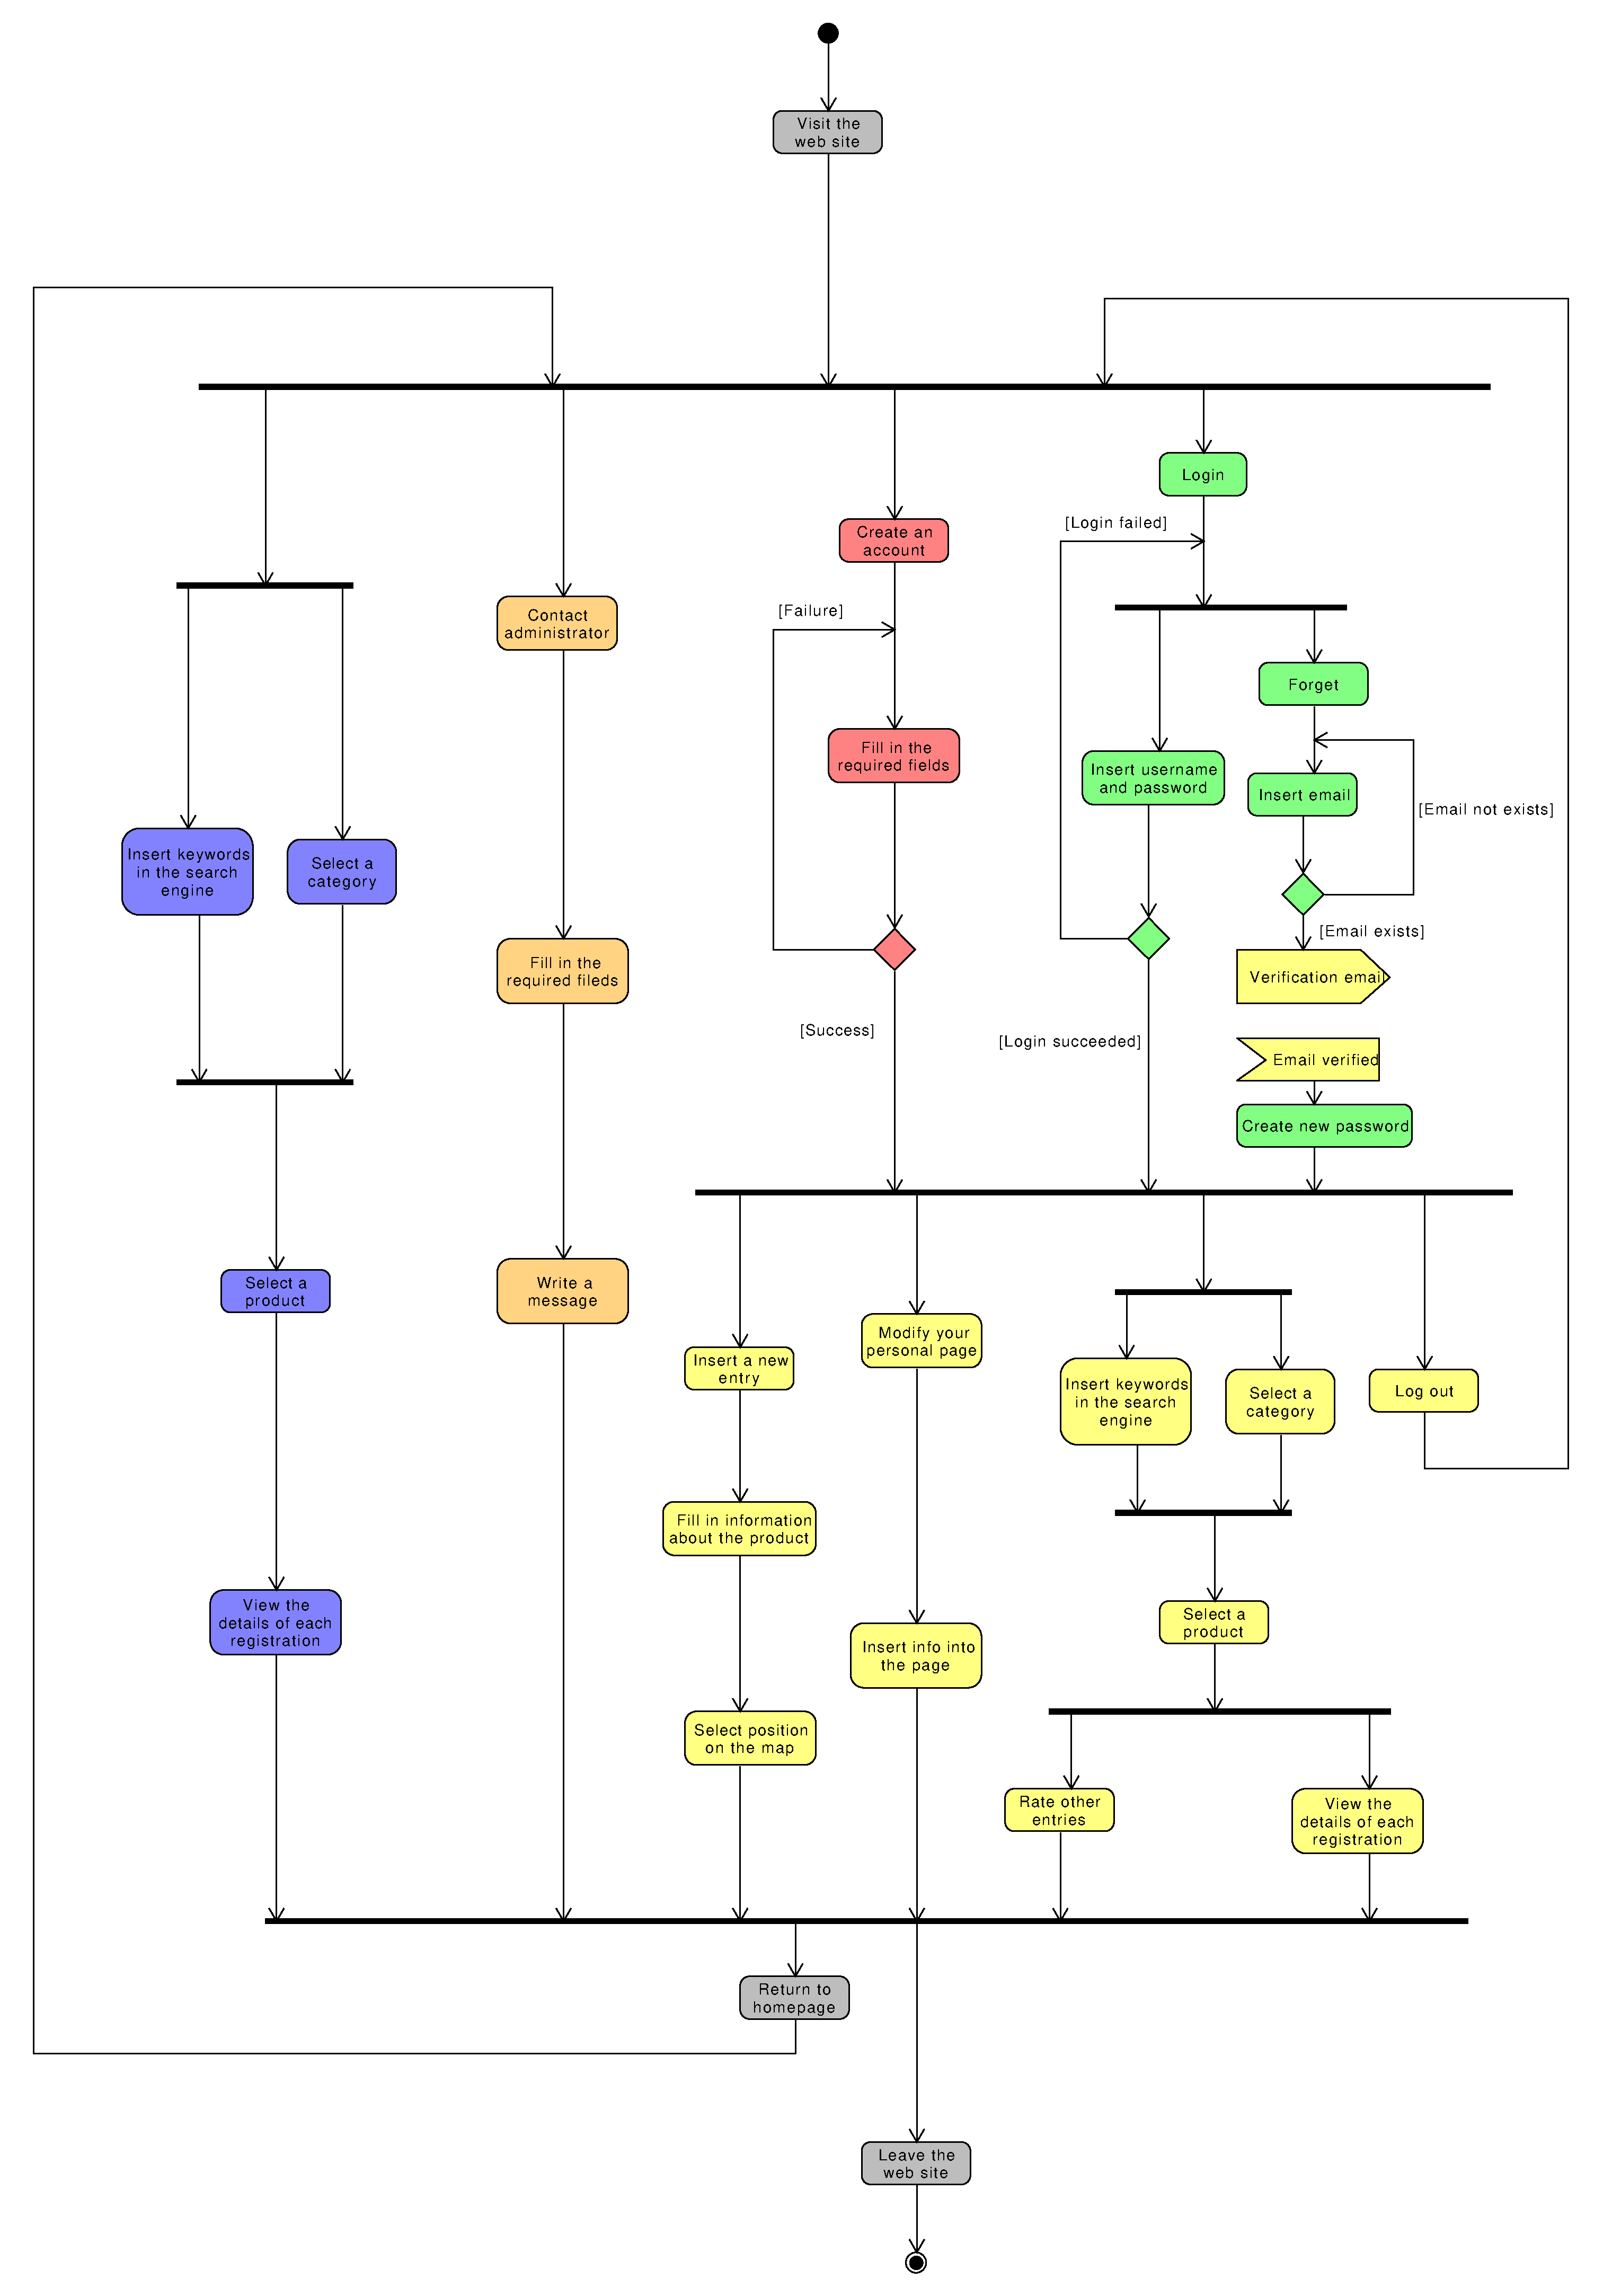
\includegraphics[scale=0.27]{userActivityDiagram.pdf}
\end{center}


\section{Αναφορές-Πηγές Πληροφοριών}

Αρχικά, οι χρήστες που συμμετέχουν στο $crowdsourcing$ αντλούν πληροφορίες από την προσωπική τους επίσκεψη στα διάφορα καταστήματα και την παρατήρηση των τιμών και των προϊόντων που συναντώνται. Επιπλεόν, μια ακόμη πηγή πληροφοριών μπορούν να αποτελέσουν άλλες δικτυακά παρατηρητήρια τιμών, αφού φυσικά πρώτα γίνει η εξακρίβωση από τη μεριά του χρήστη. Τέλος, μπορούμε να αναφέρουμε και τις καταχωρήσεις των υπόλοιπων μελών στην ιστοσελίδα, των οποίων μάλιστα η αξιοπιστία έχει εξασφαλιστεί μέσω κριτικής και της αξιολόγησης των υπόλοιπων χρηστών.

\section{Διαχειριστικές Απαιτήσεις Επιχειρησιακού Περιβάλλοντος}

\subsection{Επιχειρησιακό Μοντέλο}

Από τη σκοπιά του χρήστη δεν έχει νόημα η ανάλυση επιχειρησιακού μοντέλου, ωστόσο μπορούμε να αναφέρουμε απλοϊκά ότι ένας χρήστης επιδιώκει να εξασφαλίσει χαμηλές τιμές και υψηλή ποιότητα των παρεχόμενων υπηρεσιών, μέσω προσφορών και εκπτώσεων που ενδεχομένως προσφέρονται. 

\subsection{Περιβάλλον Διαχείρισης Πληροφοριών}

Την παρούσα χρονική περίοδο, δεν συναντάται αντίστοιχη πλατφόρμα καταγραφής προϊόντων που να βασίζεται στη μέθοδο του πληθωπορισμού. Υπάρχουν φυσικά εταιρίες, όπως είναι το $Skroutz$ που παρέχουν παρόμοιες υπηρεσίες αναζήτησης, ωστόσο βασίζονται σε μεγάλο βαθμό στη συνεργασία με κατασήματα και όχι μεμονωμένα με εθελοντές-χρήστες. Η δική μας εφαρμογή, από την άλλη καλύπτει ένα κενό της αγοράς, ενώ αξίζει να αναφερθεί, ότι ο εθελοντικός της χαρακτηρας ενισχύει την διαφάνεια, την αξιοπιστία και την αμεροληψία των καταχωρήσεων καθώς και την ποικιλία των καταστημάτων, σε σχέση με τις πιο παραδοσιακές προσεγγίσεις που ενδεχομένως ευνοούν τα μεγάλα καταστήματα που έχουν να διαθέσουν μεγαλύτερο κεφάλαιο στη διαφήμιση, έναντι μικρότερων και αναπτυσσόμενων μαγαζιών.


\section{Λειτουργικές Απαιτήσεις Επιχειρησιακού Περιβάλλοντος}

\subsection{Επιχειρησιακές διαδικασίες}

Η συλλογή και εισαγωγή προϊόντων στη βάση δεδομένων θα βασίζεται στο $barcode$.  Συγκεκριμένα, αφού ο χρήστης προσθέσει την τιμή και το τοποθεσία του καταστήματος μέσω της εφαρμογής $Google-Maps$, θα χρησιμοποιείται το $barcode$ ώστε να γίνει αναζήτηση σε μια βάση δεδομένων που θα πραγματοποιεί την ταυτοποίηση του . Στην περίπτωση που η συγκεκριμένη καταχώρηση δεν ταυτοποιηθεί, ο χρήστης καλείται να προσθέσει επιπρόσθετες πληροφορίες, όπως είναι η κατηγορία, ο κατασκευαστής και το όνομα και με βάσει αυτές τις τιμές ενημερώνεται και αντίστοιχη βάση δεδομένων ταυτοποίσης.

\subsection{Περιορισμοί}

Για έναν εγγεγραμμένο χρήστη παρατηρούνται οι ακόλουθοι περιορισμοί:
\begin{itemize}
	\item Δεν έχει πρόσβαση στα προσωπικά και ευαίσθητα δεδομένα των υπόλοιπων χρηστών, δηλαδή σε δεδομένα που ο εκάστοτε χρήστης έχει επιλέξει να μην δημοσιεύσει
	\item Δεν είναι σε θέση να διαγράψει και να τροποποιήσει με κάποιο τρόπο τις καταχωρήσεις άλλων χρηστών. Υποστηρίζεται φυσικά μηχανισμός αξιολόγησης των καταχωρήσεων, ώστε να εξασφαλίζεται η ποιότητά τους
\item Δεν μπορεί να διαγράψει άλλους χρήστες και να επέμβει με κάποιο τρόπο στο λογαριασμό τους
\item Δεν έχει τη δυνατότητα να επέμβει στη δομή και στη λειτουργικότητα της σελίδας, παρά μόνο να επικοινωνήσει με το διαχειριστή και να εκφράσει την άποψη του
\end{itemize}


\subsection{Δείκτες ποιότητας}

Για να κριθεί η ποιότητας της εφαρμογής από τη μεριά του χρήστη πρέπει να λάβουμε υπ' όψη τις ακόλουθες παραμέτρους:

	
\begin{itemize}
	\item Η απόδοση του συστήματος	ώστε να εξασφαλίζεται ταχεία πλοήγηση και αναζήτηση προϊόντων
	\item Ασφάλεια των ευαίσθητων προσωπικών δεδομένων, μέσω μεθόδων κρυπτογράφησης και της χρήσης του πρωτοκόλλου $https$
	\item Αξιοπιστια και διαθεσιμότητα του συστήματος, ώστε να εξασφαλίζεται ακεραιότητα και αδιάκοπη παροχή υπηρεσιών
	\item Φιλικό και προσαρμοστικό $UI$, προσφέροντας απλότητα και ευκολία στην πλοήγηση
	
\end{itemize}	 	


\section{Έκθεση Απαιτήσεων Χρηστών}

Οι απλοί χρήστες θα διευκολύνονταν με την ύπαρξη ευφυούς συστήματος, το οποίο θα εμφανίζει προτάσεις προϊόντων σύμφωνα με τις πρόσφατες αναζητήσεις και τις προτιμήσεις τους.  
Επιπλέον, για έναν εγγεγραμμένο χρήστη, το προσαρμοστικό αυτό σύστημα θα βασίζεται και στις προσωπικές πληροφορίες που θα έχει προσθέσει.
Θα ήταν επίσης επιθυμητό να εμφανίζονταν διαγράμματα με τις διακυμάνσεις των τιμών μεταξύ των καταστημάτων για κάθε προϊόν που επιλέγεται, αφού και η οπτικοποίηση βοηθάει στην καλύτερη κατανόηση των δεδομένων. Επιπλέον, για την περαιτέρω διευκόλυνση του χρήστη, θα ήταν εύλογο να ευνοούνται οι καταχωρήσεις που βρίσκονται σε κοντινή τοποθεσία, ενώ για την αποτελεσματικότερη αναζήτηση θα υπάρχουν πολλαπλά κριτήρια αναζήτησης.

\section{Άρχες του Προτεινόμενου Συστήματος}

Οι λειτουργικές αρχές από τη μεριά του χρήστη συνοψίζονται στα ακόλουθα σημεία:
\begin{itemize}
	\item Η πρόσθεση μεγάλου πλήθους προϊόντων για την ενημέρωση των υπόλοιπων χρηστών και κατ' επέκταση καταναλωτών σχετικά με τα διαθέσιμα χαρακτηριστικά
	\item Οι πληροφορίες που σχετίζονται με τις καταχωρήσεις να είναι έγκυρες, έγκαιρες και αμερόληπτες
	\item Η αξιόλογηση των καταχωρήσεων να είναι ανάλογη της ποιότητάς τους
	\item Να παρέχει ωφέλιμο $feedback$
\end{itemize}

\section{Περιορισμοί στο πλαίσιο του έργου}

Οι χρήστες δεν εμπλέκονται στη διαδικασία ανάπτυξης του λογισμικού.



\end{document}
